\section{Prototypical service mesh implementation}

The following chapter describes our concept of our prototypical service mesh implementation and its outcome.

\begin{figure*}
    \centering
    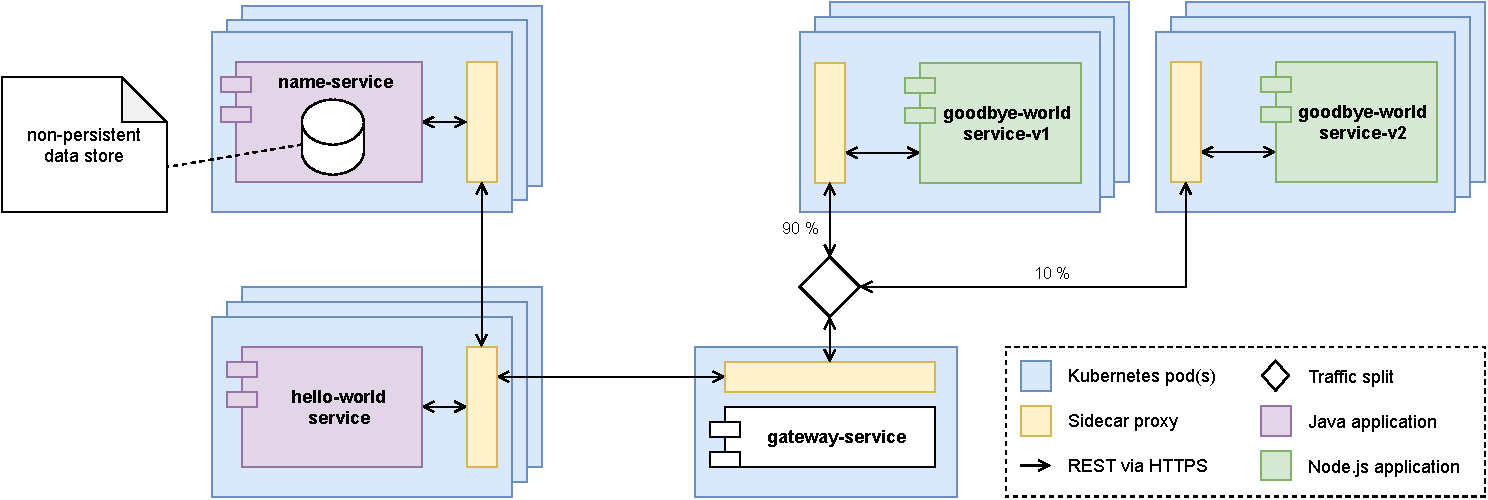
\includegraphics[width=\textwidth]{img/diagram-draft.pdf}
    \caption{Architecture overview of the PoC application}
    \label{fig:poc-overview}
\end{figure*}

\subsection{Services}

Our basic idea is to implement three simple microservice applications that communicate via REST. To prove technology independence, one service is written in Node.js, while the other two services are written in Python. Another requirement to meet is that the services have to be as simple as possible. Furthermore, the functionality of the services is intended to be as follows:

\begin{itemize}
\item \textsc{name-service}: Provides endpoint to retrieve a collection of names. It stores the names in a file or a simple array list.
\item \textsc{goodbye-world-service}: Provides endpoint to retrieve a message ``Goodbye, World!"
\item \textsc{hello-world-service}: Contacts the \textsc{name-service} and provides an endpoint that returns a ``Hello, \{name\}" message for each name object from name service.
\end{itemize}

\subsection{Showcases}

Our prototypical implementation aims to provide answers to the following five challenges of running and maintaining microservices.

\subsubsection{Encryption}

By using a service mesh, it should be shown that a encryption policy can be easily applied or removed.

\subsubsection{Canary Deployment}

To provide an example showcase for Blue/Green deployment, we implemented two versions of \textsc{goodbye-world-service} which differ minimally by the returned string. The mesh is tasked with redirecting traffic so that 90\% of all requests are made to version 1 and 10\% of requests are made to version 2.

\subsubsection{Access Policies}

Another restriction is that the \textsc{name-service} is only accessible from the \textsc{hello-world-service}.

\subsubsection{Load Balancing}
To encapsulate the services, a \textsc{gateway-service} has to be implemented. The gateway forwards the requests to the \textsc{hello-world-service} and \textsc{goodbye-world-service}. It also balances the load of requests.

\subsubsection{Central monitoring and logging}